\section{Edycja danych}
\sectionauthor{M. Gajdzis}

Po zapisaniu najnowszych danych kolejnym krokiem jest wprowadzenie niezbędnych aktualizacji dotyczących usług. W tym celu zaimplementowano dwa ekrany: pierwszy służący do wyboru usługi z listy oraz drugi, który umożliwia przeglądanie i edycję szczegółów związanych z wybraną usługą. Oba ekrany zostały zaprojektowane z myślą o intuicyjnej nawigacji i efektywnym zarządzaniu danymi.

\subsection{Ekran wyboru usługi do edycji}

% \begin{figure}[h]
% \centering
% 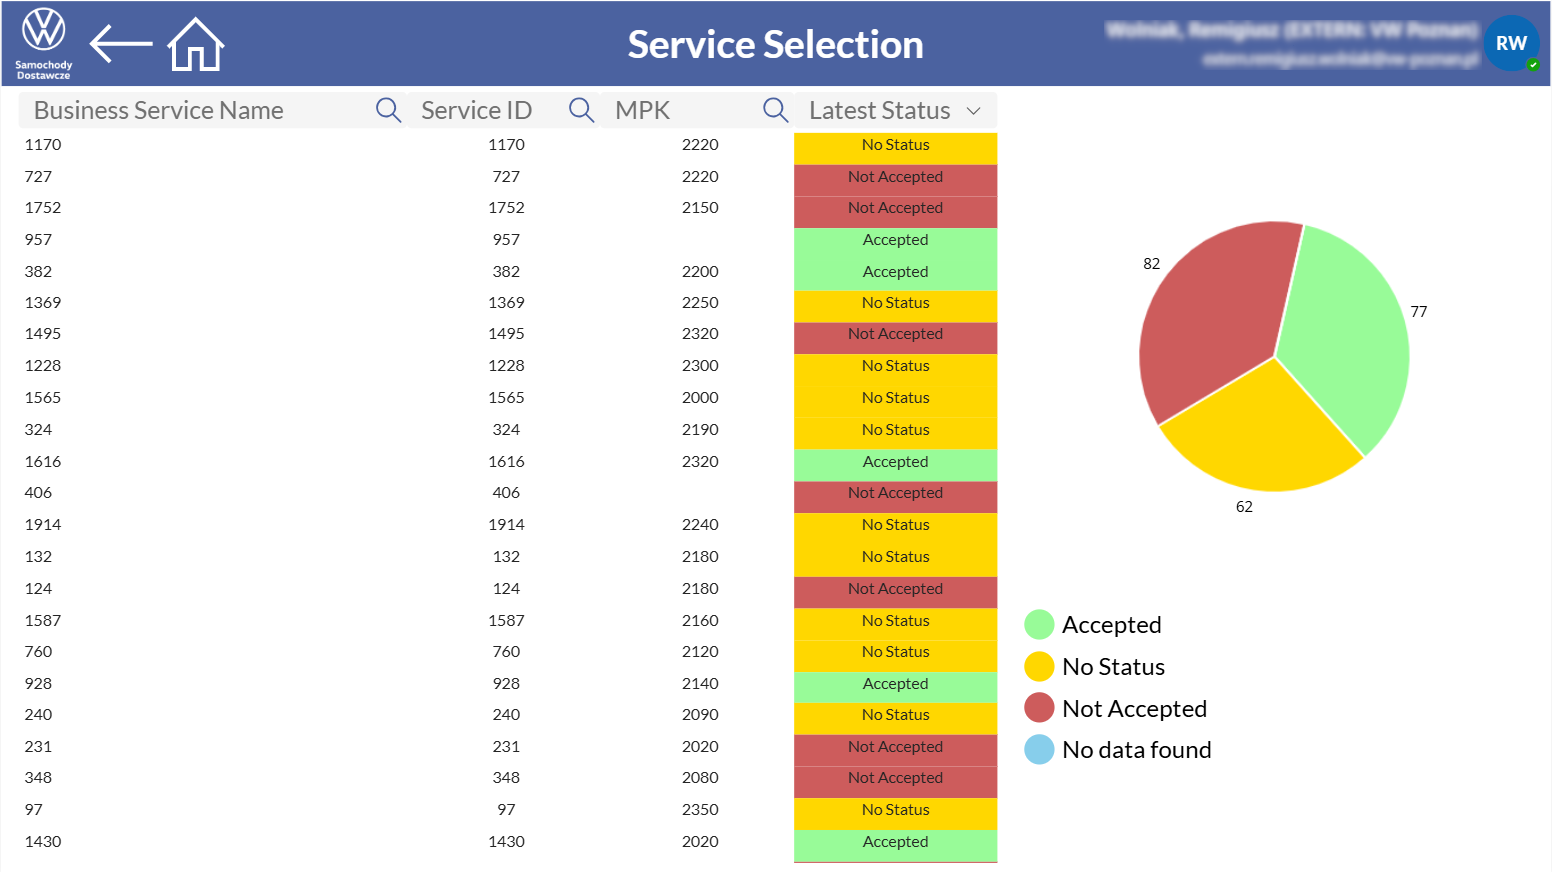
\includegraphics[width=0.9\textwidth]{figures/ServiceSelectionForm.png}
% \caption{Ekran wyboru usługi do edycji}
% \label{fig:ServiceSelectionForm }
% \end{figure}

Ekran wyboru usługi do edycji został zaprojektowany w sposób umożliwiający użytkownikom szybkie i precyzyjne wyszukiwanie oraz filtrowanie danych. Składa się z następujących elementów:

\subsubsection*{Lista wyboru serwisu}

Lista prezentuje dane pochodzące z dynamicznej kolekcji \emph{MergedData}, która została szczegółowo omówiona w poprzednim podrozdziale. Dzięki temu użytkownicy mają dostęp do aktualnych informacji bez konieczności ręcznego przeszukiwania list źródłowych.

Każdy element na liście posiada dodatkową funkcję interakcji. Po najechaniu kursorem na wybraną usługę (właściwość \emph{Hover}), element wizualnie zmienia swój wygląd -- zwęża się oraz zmienia kolor. Kliknięcie wybranego elementu przenosi użytkownika do dedykowanego ekranu edycji, który umożliwia szczegółowe zarządzanie wybraną usługą.

Dodatkowo użytkownik ma możliwość zawężenia widocznych danych poprzez zastosowanie różnych kryteriów wyszukiwania. Pola obejmują:

\begin{itemize}
    \item \textbf{Wyszukiwanie po nazwie usługi (\emph{Service Name})} -- Obsługuje częściowe dopasowania dzięki wbudowanej funkcji \emph{StartsWith}, która sprawdza, czy ciąg tekstowy zaczyna się od określonej frazy.
    \item \textbf{Filtrowanie po identyfikatorze usługi (\emph{Service ID})} -- Umożliwia precyzyjne wyszukiwanie konkretnego elementu względem jego identyfikatora (\emph{Service ID}).
    \item \textbf{Filtrowanie według miejsca powstawania kosztów (\emph{MPK})} -- Pozwala na szybkie odnalezienie danych przypisanych do konkretnego obszaru finansowego.
    \item \textbf{Filtrowanie według statusu decyzji (\emph{Accepted}, \emph{Not Accepted}, \emph{No Status})}.
\end{itemize}

Filtry te mogą być stosowane jednocześnie, co umożliwia dokładne dopasowanie wyświetlanych danych.

Warto zauważyć, że informacje dotyczące podjętej decyzji są przechowywane w bazie danych w postaci liczb całkowitych w celu szybszego przeszukiwania. Aby jednak w aplikacji widoczne były one w postaci tekstowej, zastosowano funkcję \emph{Switch}, która przypisuje odpowiednią wartość tekstową na podstawie wartości liczbowej.

\subsubsection*{Wykres kołowy}
\par
Ostatnim elementem tego ekranu jest wykres kołowy, który ilustruje podział danych według statusów decyzji.
Dane widoczne na wykresie pochodzą z listy wyboru usługi, co pozwala na uwzględnienie filtrów, np. po wprowadzeniu numeru MPK użytkownik może sprawdzić jaka część usług należąca do danego obszaru wymaga rozpatrzenia. Wartości przekazane są do właściwości \emph{Items} i uwzględniają mapowanie wartości liczbowych na tekst.



\subsection{Ekran edycji elementu}

Ekran edycji elementu prezentuje szczegółowe informacje dotyczące wybranej usługi, umożliwiając analizę danych historycznych oraz wprowadzanie nowych decyzji. Ekran składa się z kilku logicznie ułożonych sekcji, które są opisane poniżej.


\subsubsection*{Porównanie finalnych decyzji z lat poprzednich}

W górnej części ekranu umieszczona została galeria, przedstawiająca porównanie danych finansowych oraz decyzji z trzech ostatnich lat. Dane, określone we właściwości \emph{Items}, zawierają:

\begin{itemize}
    \item \textbf{Rok (Year)} -- okres, którego dotyczy dana decyzja.
    \item \textbf{Jednostka miary (Unit Of Measurement)} -- zazwyczaj ilość licencji.
    \item \textbf{Zeszłoroczne i planowane na następny rok wartości finansowe} -- \emph{Current Year Plan} oraz \emph{Next Year Plan}.
    \item \textbf{Różnice w finansach (Difference)} -- różnica między zeszłorocznymi i potencjalnymi przyszłymi kosztami.
    \item \textbf{Status końcowej decyzji (Final Decision)} -- decyzje dotyczące finalnej decyzji z danego roku (\emph{Accepted, Not Accepted, No Status}).
\end{itemize}


% \subsubsection*{Link do instrukcji obsługi}

% Poniżej tabeli z porównaniem decyzji znajduje się link do dedykowanej instrukcji obsługi usługi. Za pomocą linku użytkownik posiada dostęp do szczegółowych informacji na temat zasad korzystania z danej usługi, co może być przydatne podczas edycji danych lub wprowadzania nowych decyzji.

Galeria ta jest interaktywna. Oznacza to, że po kliknięciu na wybrany wiersz, wyświetlana jest kolejna galeria, która zawiera szczegółowe informacje na temat poszczególnych indykacji z wybranego roku.

\subsubsection*{Porównanie tegorocznych indykacji}

Druga galeria wyświetla następujące informacje:
\begin{itemize}
    \item \textbf{Numer indykacji (Indication Number)},
    \item \textbf{Komentarze} -- w tym \emph{Internal Comment, Comment PZ to WOB, Comment K-DES},
    \item \textbf{Data i autor komentarza},
    \item \textbf{Status decyzji (Decision)}.
\end{itemize}

Aby uniknąć problemu z czytelnością długich komentarzy, które nie mieszczą się w przeznaczonych komórkach, zaimplementowano możliwość kliknięcia na element. Skutkuje to ustawieniem wartości zmiennej \emph{ShowCommentPopup}, odpowiedzialnej za widoczność okna dialogowego, na wartość \emph{True}. W oknie tym wyświetlany jest autor, data wprowadzenia oraz pełna treść komentarza. Dane dotyczące komentarza przekazywane są w zmiennej tablicowej \emph{SelectedComment}, która aktualizowana jest w momencie wybrania komórki z komentarzem.

\subsubsection*{Formularz do uzupełnienia danych}

Na samym dole strony znajduje się formularz umożliwiający wprowadzenie nowych danych lub aktualizację istniejących rekordów. Formularz zawiera pola takie jak:
\begin{itemize}
    \item \textbf{Rok (\emph{Year})} -- pole typu \emph{Dropdown}, zawiera dane z kolekcji \emph{colYears} tworzonej przy uruchomieniu aplikacji,
    \item \textbf{Numer indykacji (\emph{Indication Number})} -- pole typu \emph{Dropdown}, zawiera dane z kolekcji \emph{colNumbers} tworzonej przy uruchomieniu aplikacji,
    \item \textbf{Komentarze} -- pole \emph{TextInput} (wprowadzania tekstu),
    \item \textbf{Status decyzji (\emph{Decision})} -- pole typu \emph{Dropdown}. Dane we właściwości \emph{Items}, zdefiniowane są jako \emph{["Accepted", "No Status", "Not Accepted"]}.
    \item \textbf{Data} -- kontrolka \emph{DatePicker}, która umożliwia wybór daty poprzez wyświetlenia kalendarza,
    \item \textbf{Autor} -- pole \emph{ComboBox}, umożliwia wybór autora z listy pracowników. Lista ta pobierana jest poprzez connector \emph{Office365Users}\footnote{\emph{Office365Users} -- konektor pozwalający na dostęp do listy zawierającej informacje na temat użytkowników takie jak imię, nazwisko, dane kontaktowe lub dział.}, który zawiera informacje na temat wszystkich użytkowników infrastruktury firmy.
\end{itemize}


\subsubsection*{Przycisk zapisu}


Ostatnim elementem na tym ekranie jest przycisk \emph{Save}, który umożliwia zapisanie wprowadzonych zmian. Mechanizm ten:

\begin{itemize}
    \item Sprawdza istnienie wcześniejszych indykacji, aby upewnić się, że zachowana jest poprawna kolejność numeracji.
    \item W przypadku istniejącego wpisu -- uzupełnia dane przy użyciu funkcji \emph{Patch}.
    \item W przypadku nowego wpisu -- tworzy nowy rekord przy użyciu funkcji \emph{Defaults}.
    \item Resetuje pola formularza oraz odświeża dane na ekranie, aby uwzględnić ostatnie zmiany.
    \item Informuje użytkownika o powodzeniu lub błędach operacji za pomocą komunikatów (\emph{Notify}).
\end{itemize}

\subsection{Listing kodu}

Listing \ref{lst:SaveFormCode} przedstawia fragment kodu odpowiedzialny za zapisywanie danych w formularzu edycji, który jest wywoływany po kliknięciu przycisku \emph{Save}. Kod ten odpowiedzialny jest za zapisanie informacji z formularza w bazie danych.

\begin{lstlisting}[language=PowerFx, caption={Kod zapisywania danych w formularzu edycji}, label=lst:SaveFormCode]
    If(
        // Dla indykacji nr 1
        IndicationNo_Dropdown.Selected.Value = 1;
        
        // Sprawdź czy istnieje już pierwsza indykacja
        If(
            !IsBlank(
                LookUp(
                    Lista_Indykacji;
                //elementy listy   )
            );
            // W przypadku istnienia - aktualizacja istniejącego rekordu
            Set(
                TempOutput;
                Patch(
                    Lista_Indykacji;
                    LookUp(
                        Lista_Indykacji;
                        [...] //elementy listy  )
            Notify("A record has been successfully updated!");
            
            // Jeśli rekord nie istnieje utwórz nowy
            Set(
                TempOutput;
                Patch(
                    Lista_Indykacji;
                    [...] //elementy listy
                )
            );;
            Notify("The record has been successfully created!")
\end{lstlisting}